\documentclass[11pt,a4paper]{report}
\usepackage[english]{babel}
\usepackage[utf8]{inputenc}
\usepackage[T1]{fontenc}
\usepackage{glossaries}
\usepackage{graphicx}
\usepackage{hyperref}
\usepackage{wrapfig}
\usepackage{float}
\usepackage{natbib}
\usepackage{listings}
\usepackage{caption}
\usepackage{subcaption}

\usepackage{color}
 
\definecolor{codegreen}{rgb}{0,0.6,0}
\definecolor{codegray}{rgb}{0.5,0.5,0.5}
\definecolor{codepurple}{rgb}{0.58,0,0.82}
\definecolor{backcolour}{rgb}{0.95,0.95,0.92}

\graphicspath{ {images/} }

\newcommand{\HRule}{\rule{\linewidth}{0.5mm}}
\setlength\parindent{0pt} 

\let\olditemize\itemize
\renewcommand{\itemize}{
  \olditemize
  \setlength{\itemsep}{1pt}
  \setlength{\parskip}{0pt}
  \setlength{\parsep}{0pt}
}

\title{\textbf{Internet Service Provider ARA Project} \\Arquitectura de Redes Avançada \\Universidade de Aveiro}
\author{Diogo Silva 60337 \and Eduardo Sousa 68633 }

\begin{document}
\begin{titlepage}
\begin{center}
\HRule \\[0.4cm]
{ \huge \bfseries Internet Service Provider ARA Project \\[0.4cm] }
\HRule \\[1.5cm]
\textsc{\LARGE Universidade de Aveiro}\\[1.5cm]
\textsc{}\\[1.5cm]
\textsc{Diogo Silva 60337 \\Eduardo 68633 }
\end{center}
\end{titlepage}
\maketitle
\tableofcontents

\lstdefinestyle{mystyle}{
    backgroundcolor=\color{backcolour},   
    commentstyle=\color{codegreen},
    keywordstyle=\color{magenta},
    numberstyle=\tiny\color{codegray},
    stringstyle=\color{codepurple},
    basicstyle=\footnotesize,
    breakatwhitespace=false,         
    breaklines=true,                 
    captionpos=b,                    
    keepspaces=true,                 
    numbers=left,                    
    numbersep=5pt,                  
    showspaces=false,                
    showstringspaces=false,
    showtabs=false,                  
    tabsize=2
}
\lstset{style=mystyle}

\chapter{Basic Mechanisms and BGP}

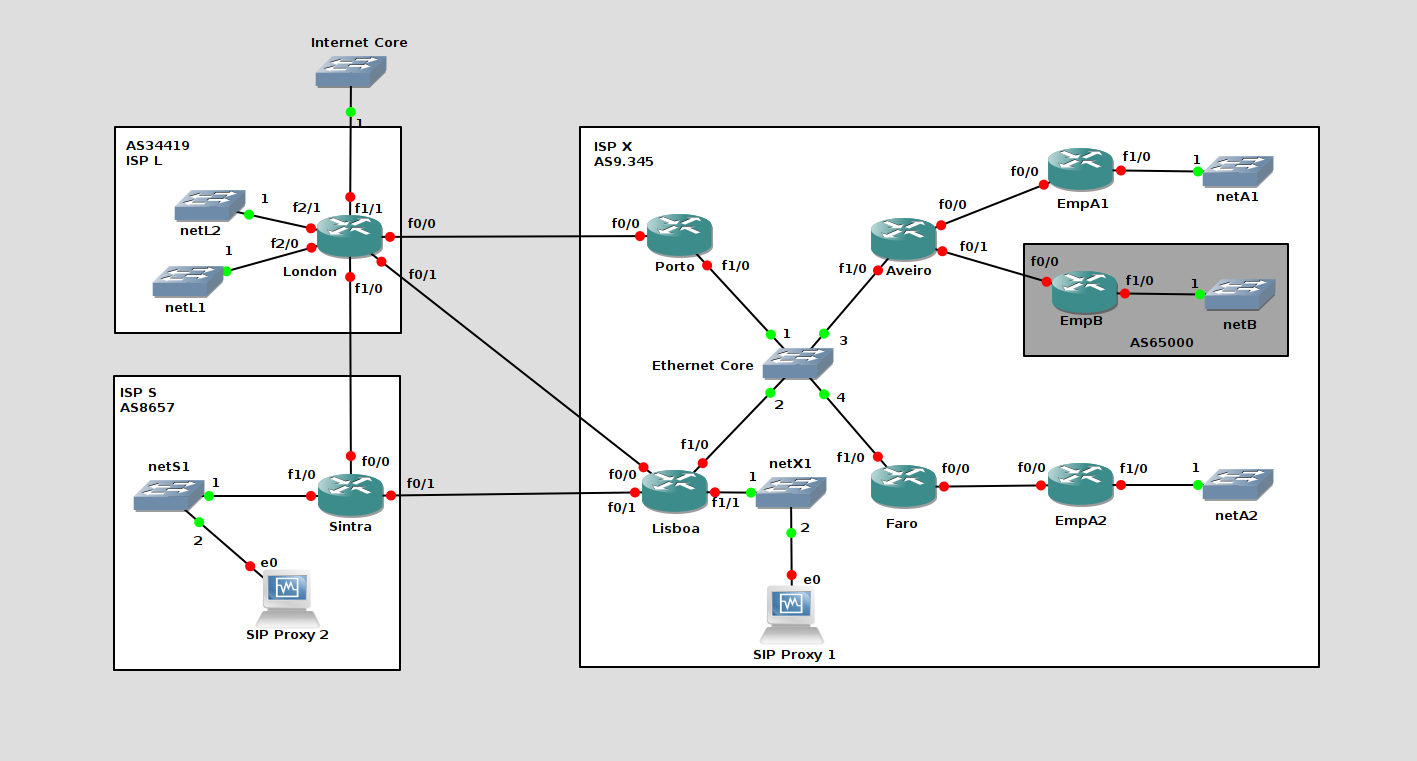
\includegraphics[scale=0.3]{network}

\section{Internal BGP \& OSPF Redistribution}
\#EDUARDO
\section{External BGP}
\#EDUARDO
\section{Private AS}
\#EDUARDO

\section{Routing Constraints}

Neste projecto todas as restrições de routing apresentadas a seguir foram efectuadas usando route-map para efectuar a respectiva regra, ou negar a rota, ou aumentar a local preference da rede anunciada no iBGP.

\subsection{Internet Traffic}

``IP traffic towards Internet should be preferably routed via ISP S (Lisboa).''
\newline

Se a rota pertence à internet incrementa-se a preferência local (podia-se ter usado 0.0.0.0 para representar qualquer outra rede externa, ou seja, internet). No trecho de código seguinte podemos ver que se o ip da internet se verificar, coloca uma preferência local acima da default, caso não seja, anuncia a rota como veio.

\begin{lstlisting}[caption=Route-map para a Internet]
access-list 5 permit 8.8.8.0 0.0.0.255

route-map INTERNET_LP permit 10
 match ip address 5
 set local-preference 200

route-map INTERNET_LP permit 20
\end{lstlisting}

Como se pretende dar mais preferência à ligação entre Sintra e Lisboa quando o tráfico vai para a internet, aplica-se o route-map a todas as rotas anunciadas por Sintra a Lisboa, sendo que se alguma dessas rotas anunciadas por Sintra pertencer a internet, a preferência local será aumentada.\\

\begin{lstlisting}[caption=Route-map da Internet no Neighbor Sintra no Router de Lisboa]
router bgp 9.345
 address-family ipv4
  ...
  neighbor 4.20.20.13 route-map INTERNET_LP in
\end{lstlisting}

\subsection{Net L1 and Net L2 Preferences}

``IP traffic towards netL1 and netL2, should be preferably routed via Porto from Aveiro, and via Lisboa from Faro.''
\newline

Definiu-se a seguinte route-map em Aveiro e Faro, tendo em conta que ambos querem aumentar a preferência para a route-map na netL1 e netL2, a única diferença é por onde querer ir (só muda onde é aplicada a route-map), então definiu-se a mesma para os dois.

\begin{lstlisting}[caption=Route-map para a netL1 e netL2]
access-list 10 permit 82.84.100.0 0.0.0.255
access-list 10 permit 82.84.200.0 0.0.0.255

route-map LNET_LP permit 25
 match ip address 10
 set local-preference 210
route-map LNET_LP permit 30
\end{lstlisting}

Depois de definida a route-map, aplicou-se a rota ao neighbor respectivo.

Se Aveiro receber uma rota anunciada pelo Porto que cumpra a route-map, aumenta-lhe a perferência. Em Faro caso receba uma rota anunciada por Lisboa que cumpra a route-map, aumenta-lhe a preferência local.

Isso fez-se através do seguinte código.\\
\begin{lstlisting}[caption=Route-map LNET\_LP no Neighbor Porto no Router de Aveiro]
  neighbor 192.172.100.1 route-map LNET_LP in
\end{lstlisting}

\begin{lstlisting}[caption=Route-map LNET\_LP no Neighbor Lisboa no Router de Faro]
  neighbor 192.172.100.2 route-map LNET_LP in
\end{lstlisting}

\subsection{SIP Proxy 2 Traffic}

``IP traffic for remote SIP proxy 2 (to network netS1) should be routed only via Lisboa using the direct peering link to ISP S.''
\newline

Para fazer com que Lisboa -> Sintra fosse o único peering possível do ISP X para a NetS1, optou-se pela estratégia oposta, negar todas as saídas possíveis, ou seja, tudo o que anunciar a NetS1 e que não seja aquele link não é aceite. Sendo definida a seguinte rota:\\

\begin{lstlisting}[caption=Route-map SIP\_ROUTE para cancelar rotas]
access-list 6 permit 200.1.100.0 0.0.0.255

route-map SIP_ROUTE deny 11
 match ip address 6
route-map SIP_ROUTE permit 21
\end{lstlisting}

Sendo que foi preciso definir nos neighbors as rotas, neste caso, em Lisboa e Porto, rotas para a NetS1 recebidas pelo link de London.\\

\begin{lstlisting}[caption=Cancelar rota para NetS1 recebida em Lisboa por London]
neighbor 4.20.20.5 route-map SIP_ROUTE in
\end{lstlisting}

\begin{lstlisting}[caption=Cancelar rota para NetS1 recebida no Porto por London]
neighbor 4.20.20.1 route-map SIP_ROUTE in
\end{lstlisting}

\subsection{Non-Transit ISP-X}

Para efectuar o Non-Transit foi preciso definir uma verificação no as-path, se o AS-PATH for vazio, ou contiver apenas o AS 65000 (privado) significa que é uma rota interna e pode ser anunciada para que os outros saibam que aquele neighbor pode ser usado para chegar a rede anunciada, sendo que redes que contenham outros AS-PATH (Sistemas autonomos externos não serão anunciados para fora).\\

Teve-se de verificar para o AS 65000 porque ele atravessa pelo AS 9.345 para sair para London ou Sintra, e o rm-private-as é apenas retirado depois da validação das route-maps definidas no neighbor.\\

Sendo que se usou a seguinte route-map em todas as saídas possíveis do AS 9.345:

\begin{lstlisting}[caption=Tornar ISP X num AS Non-Transit]
ip as-path access-list 4 permit ^$
ip as-path access-list 4 permit ^65000$
route-map NON_TRANSIT permit 10
 match as-path 4
\end{lstlisting}

Sendo depois aplica-se esta route-map em Lisboa e no Porto em todos os neighbors ao anunciar rotas para fora (neighbor VIZINHO route-map NON\_TRANSIT out)

\section{Changes for IPv6}
\#EDUARDO

\chapter{MPLS}
\#DIOGO
\section{MPLS Tunnel for SIP Traffic}
\section{MPLS VPN}


\chapter{VoIP SIP}

Neste projeto foi pedido que existisse um serviço de SIP-VoIP para todos os clientes empresariais do ISP X. Esse serviço VoIP deve fornecer conetividade entre todos os clientes empresariais, bem como fornecer compatibilidade com chamadas oriundas de PTSN, encaminhadas pelo SIP Proxy 2. O serviço de VoIP deve também encaminhar as chamadas para redes externas utilizando o SIP Proxy 2.

\section{Internal Extensions}

A configuração dos clientes é a seguinte:

\begin{lstlisting}[caption=SIP Proxy 1 - /etc/asterisk/sip.conf]
[EmpA1]
type=friend
host=dynamic
secret=labcom
context=phones
allow=all

[EmpA2]
type=friend
host=dynamic
secret=labcom
context=phones
allow=all

[EmpB]
type=friend
host=dynamic
secret=labcom
context=phones
allow=all
\end{lstlisting}

Apenas existe uma conta por empresa, para ser possível testar a conetividade entre elas. Na realidade poderiam existir muitas mais sem que existem problemas.\\

De seguida configurou-se a extensões dos clientes, sendo elas:

\begin{lstlisting}[caption=SIP Proxy 1 - /etc/asterisk/extensions.conf]
[phones]
exten => 1000,1,Answer(500)
exten => 1000,2,PlayBack(demo-congrats)
exten => 1000,3,PlayBack(vm-goodbye)
exten => 1000,4,HangUp()

exten => 2000,1,Dial(SIP/EmpA1)
exten => 2000,2,voicemail(3000@corporations_voicemail)
exten => 2000,3,PlayBack(vm-goodbye)
exten => 2000,4,HangUp()

exten => 2001,1,Dial(SIP/EmpA2)
exten => 2001,2,voicemail(3001@corporations_voicemail)
exten => 2001,3,PlayBack(vm-goodbye)
exten => 2001,4,HangUp()

exten => 2002,1,Dial(SIP/EmpB)
exten => 2002,2,voicemail(3002@corporations_voicemail)
exten => 2002,3,PlayBack(vm-goodbye)
exten => 2002,4,HangUp()

exten => 3000,1,voicemail(3000@corporations_voicemail)
exten => 3001,1,voicemail(3001@corporations_voicemail)
exten => 3002,1,voicemail(3002@corporations_voicemail)
\end{lstlisting}

A extensão 1000 serve para testar a conetividade com o servidor. 
A extensão 2000 é a extensão do polo 1 da empresa A. 
A extensão 2001 é a extensão do polo 2 da empresa A. 
A extensão 2002 é a extensão da empresa B. 
As extensões 3000, 3001 e 3002 dão acesso ao voicemail das empresas.
Todas as extensões 2000, 2001 e 2002 caso estejam ocupadas vão parar ao voicemail.\\

As configurações do voicemail são as seguintes:

\begin{lstlisting}[caption=SIP Proxy 1 - /etc/asterisk/voicemail.conf]
[corporations_voicemail]
3000 => 1212,EmpA1
3001 => 1212,EmpA2
3002 => 1212,EmpB
\end{lstlisting}


\section{PTSN Calls Support}

As chamadas provenientes da rede PTSN vão utilizar a seguinte configuração para serem reencaminhadas para as respetivas empresas.

\begin{lstlisting}[caption=SIP Proxy 1 - /etc/asterisk/extensions.conf]
[phones]
...
exten => _2341000XX,1,Dial(SIP/EmpA1)
exten => _2341000XX,2,voicemail(3000@corporations_voicemail)
exten => _2341000XX,3,PlayBack(vm-goodbye)
exten => _2341000XX,4,HangUp()

exten => _2891001XX,1,Dial(SIP/EmpA2)
exten => _2891001XX,2,voicemail(3001@corporations_voicemail)
exten => _2891001XX,3,PlayBack(vm-goodbye)
exten => _2891001XX,4,HangUp()

exten => _2341002XX,1,Dial(SIP/EmpB)
exten => _2341002XX,2,voicemail(3002@corporations_voicemail)
exten => _2341002XX,3,PlayBack(vm-goodbye)
exten => _2341002XX,4,HangUp()
\end{lstlisting}

O underscore indica o inicio do padrão que queremos utilizar e o X indica números de 0 a 9. De resto a configuração é semelhante a anterior.

\section{Forward to SIP Proxy 2}

Para fazer reencaminhar as chamadas VoIP para redes externas é preciso alterar as configurações dos dois servidores SIP.

\begin{lstlisting}[caption=SIP Proxy 1 - /etc/asterisk/sip.conf]
...
[Server2]
type=peer
host=200.1.100.2
secret=labcom
username=Server1
\end{lstlisting}

\begin{lstlisting}[caption=SIP Proxy 2 - /etc/asterisk/sip.conf]
[Server1]
type=peer
host=192.172.100.130
secret=labcom
context=phones
\end{lstlisting}

\begin{lstlisting}[caption=SIP Proxy 1 - /etc/asterisk/extensions.conf]
...
exten => _X!,1,Dial(SIP/${EXTEN}@Server2,10)
exten => _X!,2,HangUp()
\end{lstlisting}

\begin{lstlisting}[caption=SIP Proxy 2 - /etc/asterisk/extensions.conf]
[phones]
exten => _X!,1,Answer(500)
exten => _X!,2,PlayBack(demo-congrats)
exten => _X!,3,PlayBack(vm-goodbye)
exten => _X!,4,HangUp()
\end{lstlisting}

No servidor 1 foi preciso criar um peer para permitir que o mesmo se consiga ligar ao servidor 2. Foi também preciso criar uma nova regra nas extensões do servidor 1 que reencaminhe todas as chamadas VoIP com destino em extensões externas para o servidor 2, assim sendo foi criado o padrão \_X!, onde o underscore indica o inicio do padrão, o X indica qualquer número e o ! todas as extensões não definidas anteriormente. Caso se encontre alguma chamada para uma extensão deste tipo, o servidor 1 deve fazer uma SIP URI dial para o servidor 2 para onde envia a extensão.\\
No servidor 2 foi preciso criar um peer para indicar que o servidor 1 se vai ligar a ele. As extensões são idênticas às definidas anteriormente.

\lstlistoflistings
\bibliographystyle{plain}
\bibliography{proj2}

\end{document}
